
\section{Architectures Of Deep Neural Networks}


When it comes to building a neural network, one has to establish an
architecture or an arrangement of layers and how they connect with each other.
It is particularly important, when the network increases in complexity. Object
classification + localization being a demanding task for a network to solve,
we have adopted a published and well-tested architecture for the task --
ResNet. The particular architecture we have tried to imitate titled 
\textit{DECOLLE}, was first developed by \citeA{kaiser2018synaptic} and later
enhanced by \citeA{barchid2021deep}. \textit{DECOLLE} Neural Network adopts 
properties of classical ResNet model architecture as well as a pyramidal structure that
was proposed by \citeA{pyramid}. 


\subsection{ResNets}



To begin with the cornerstone of our architecture -- ResNet, it was named for its property,
of convolutional layers of the network that are residually connected with each other using
shortcut connections (\citeA{resnet}).
According to the authors of the original paper on ResNets,
addition of residual connections improves model's convergence, or ability for
model's loss to move towards a minimum with a decreasing trend. Meanwhile,
ResNets converge faster than their plain counterparts, the complexity of 
ResNets is much lower than complexity of well established Visual Geometry
Group (VGG) Networks given the same depth (3.6 billion FLOPs (Float Point 
Operations) vs. 19.6 billion FLOPs) (\citeA{resnet}). 

\subsection{Comparing Model Performance}
To compare networks' performance one has to understand how it is measured and what
constitutes an accurate model. For the task of object detection/localization accuracy
of the model at predicting class of the object in the image is not enough. Thus,
two additional performance metrics have been adapted : Mean Average Precision (mAP) and
Intersection of Union (IoU). Firstly, Mean Average Precision for the purposes of Object
Detection is well-defined in the paper by \citeA{evaluation}. According to the authors,
mAP is mean of Average Precision of the model for all the classes in the dataset. It is
calculated using the following equation.


\begin{equation}
	\textbf{mAP} = \frac{1}{N} * \sum_{i = 1}^{N} \textbf{AP}_i
\end{equation}

\begingroup
\fontsize{7pt}{9pt}\selectfont
\begin{enumerate}
	\item[]  \begin{center} AP = Average Precision, \end{center}
	\item[] \begin{center}  N = number of classes. \end{center}
\end{enumerate}
\endgroup


Next, IoU is the area of overlap of ground-truth boxes and the model's detected box output,
the higher the IoU the better performance of the model. Intersection of Union can be 
represented as follows:

\begin{equation}
	\textbf{IoU} = |A \cap B| \div  |A \cup B| = |I| \div |U|
\end{equation}

\begingroup
\fontsize{7pt}{9pt}\selectfont
\begin{enumerate}
	\item[]  \begin{center} I = Intersection area, \end{center}
	\item[] \begin{center}  U = Union area. \end{center}
\end{enumerate}
\endgroup


\subsection{Pyramidal Architecture of Neural Network}


Pyramidal structure of a Neural Network refers to the shape of the layers as the model
gets deeper. With each layer dimensions of convolutional layers shrink (usually in half).
For example, the first convolutional layer would have input dimension equal to number of
channels in the image (3 channels in case of RGB images vs. 1 for grayscale) and the output
dimension of 512, with next layer input equal to previous layer's output. Second layer
would have the dimension of 256 (half of previous layer's output) and so on (\citeA{pyramid}).

For the purposes of our network, pyramidal structure of neural network is leveraged using
Encoder-Decoder model. When image is passed through the shrinking layers of the Encoder
Pyramid, it loses resolution as well as contextual information, however when the image
leaves the encoder and is located in the hidden state it is fully comprised of
the semantic information about the image (What object is on the picture and where it is
located). Furthermore, in order to localize an object on the image that model has never 
encountered before, it has to be able to place the semantic information in context. 
This is where Decoder comes into play, being the reverse of an Encoder, the convolutional
layers of decoder double in size until desired dimensions. The decoder is residually
connected to encoder, and thus it gains contextual information about the image through
every pass of a layer.

At the end, in order to extract meaningful, last decoder layer is connected
to fully connected linear layers that  output predicted class as well as
detected box coordinates.





\subsection{Architecture of the Model Used}

\begin{figure}[h]
	\begin{center}
		\scalebox{0.4}{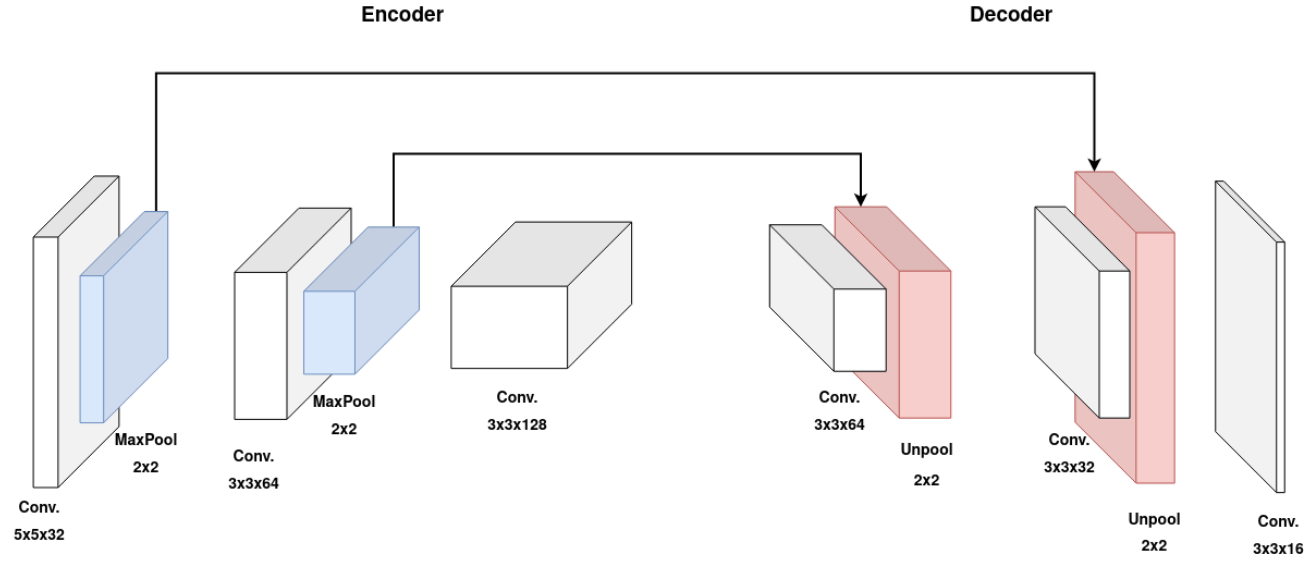
\includegraphics{barchid_SED.png}}
	
	\end{center}
	\caption{Sketch of the model's architecture. White layers represent convolutional layers,
	blue represent pooling layers, and red unpooling layers}
\end{figure}

Architecture developed by \citeA{barchid2021deep} was the target to replicate. The model is based
on Encoder-Decoder architecture with residually connected layers akin to ResNets. Encoder and 
Decoder follow the pyramidal architecture that was discussed earlier. 




\section{Implementation}

\subsection{PyTorch}

The main package that allowed us to develop such a complex model was PyTorch. PyTorch
is an open-source a machine learning/deep learning library and framework for Python 
that allows user to develop and ship high performance models (\citeA{pytorch}). This library
eliminates the need from scratch development of the most important methods in machine learning,
such as activation functions, model architecture assembly, 


\subsection{Spiking Neurons}

Given the complexity of Spiking Neural Networks and the integration of Leaky-Integrate-and-Fire
into the network, we used a package that allows to use LIF within a PyTorch model -- 
\href{https://snntorch.readthedocs.io/en/latest/snntorch.html}{\textit{snnTorch}}. 
snnTorch also allowed us to integrate backpropogation for spiking neural networks
with one line. Indeed, to use LIF in your model only need to use one line in model
definition.

\begin{lstlisting}[language=Python, caption=Leaky-Integrate-and-Fire using snnTorch]
	import snntorch as snn
	spike_grad = surrogate.fast_sigmoid(slope=25)
	beta = 0.5

	lif1 = snn.Leaky(beta=beta, spike_grad=spike_grad)

\end{lstlisting}

\subsection{Membrane Potentials}

We have previously discussed the difficulty of implementing membrane potentials into spiking neural networks. Thankfully, snnTorch provides a method that stores that information for the duration of an epoch.

\begin{lstlisting}[language=Python, caption=snnTorch Implementation of Membrane Potentials]
import snntorch as snn
import torch as nn

spike_grad = surrogate.fast_sigmoid(slope=25)
beta = 0.5

def mock_layer(input):

    conv1 = nn.Conv2d(in_channels, 32, kernel_size=7)
    lif1 = snn.Leaky(beta=beta, spike_grad=spike_grad)

    out = self.conv1(input)
    out = F.max_pool2d(out, 2)
    spike, membrane_potential = self.lif1(out, membrane_potential)
		return spike, membrane_potential

\end{lstlisting}


\section{Challenges}

\subsection{What}

With the number of operations required to train the model to complete the task of object
localization, it was clear since the beginning that a lot of computational power was required. A number
of steps was required in order to make this project plausible the scope of this course.

First challenge in implementation of the model was difficulty to replicate the 
\citeA{barchid2021deep} paper given the lack of description on the implementation in the 
paper as well non-existence of public repository with the code for their model.